\section{Hidden States as an Object of Study}
\label{sec:hidden-states}

The emitted tokens are the only part of a forward pass that the application calling the model observes, but the pass also produces one vector per layer and per position. These vectors are the object of study of this section.

\subsection{What a hidden state is}
\label{subsec:hidden-states}

The \emph{hidden state} of a model at layer $\ell$ and position $i$ is the vector produced at that position by block $\ell$. This vector is the value carried into block $\ell+1$. It is written here as
\begin{equation}
    h^{(\ell)}_i ,
    \qquad \ell = 1, \dots, L ,
    \qquad i = 1, \dots, n ,
\end{equation}
where $L$ is the number of blocks and $n$ is the number of tokens in the input. Each $h^{(\ell)}_i$ is a vector of dimension $d_{\mathrm{model}}$. One forward pass therefore produces $L \times n$ such vectors.

\begin{figure}[ht]
	\centering
	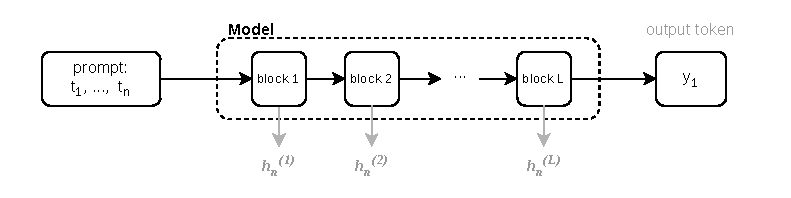
\includegraphics[width=0.9\textwidth]{images/hidden-states-ex.pdf}
	\caption[Hidden states across blocks]{The hidden states written at the last prompt token, $h^{(1)}_n, \dots, h^{(L)}_n$.}
	\label{fig:hidden-states}
\end{figure}

The set of these vectors is the representation that the model forms of the input while it processes it. At a fixed position, the vectors at increasing $\ell$ are successive states of the same representation, since each block reads the value produced by the previous one and writes an updated value into it. The prediction is refined block by block as a result \cite{gevaTransformerFeedForwardLayers2021, belroseElicitingLatentPredictions2025}. The content of these states depends on the layer. Ethayarajh measured how much the representation of a word varies with the context it appears in, on ELMo, BERT and GPT-2, and reported that the higher the layer, the more context-specific the representation is \cite{ethayarajhHowContextualAre2019}. After correcting for a property of these representations called anisotropy (Section~\ref{subsec:anisotropy}), Ethayarajh computed the first principal component of a word's representations across its contexts, a single fixed vector, and measured how much of the variation in those representations it explained. In every layer of the three models, on average, that vector explained less than 5\% of the variance in the word's representations across contexts. A word therefore has no small set of fixed senses that the model picks from: its representation differs in almost every context \cite{ethayarajhHowContextualAre2019}.

The last hidden state, $h^{(L)}_n$, is the vector to which the unembedding of Section~\ref{subsec:unembedding} is applied.

\subsection{Probing as a method}
\label{subsec:probing-method}

Reading a property off the hidden states is defined as \emph{probing}. A \emph{probe} is a classifier trained to predict a property of interest from the representations of a frozen model, and trained independently of the model itself \cite{alainUnderstandingIntermediateLayers2018a}. The representations are the input of the classifier and the property is its label, so the accuracy of the probe measures the degree to which the property is recoverable from the representation it is fitted on \cite{alainUnderstandingIntermediateLayers2018a}. Probing classifiers have become one of the main methods for analyzing neural models of natural language processing, and their methodological limitations have been reviewed critically \cite{belinkovProbingClassifiersPromises2021a}.

A probing result is limited both by what a high accuracy can establish and by the probe itself. A high accuracy establishes that a property is decodable from a representation. It does not establish that the model uses the property to produce its output \cite{belinkovProbingClassifiersPromises2021a}. Orgad et al. found that a model can encode the correct answer and consistently generate an incorrect one; this is the empirical form of the same distinction, since the property is present in the representation while the output does not reflect it \cite{orgadLLMsKnowMore2025}. The probe itself is a further limitation. A classifier with enough capacity can memorize the labels of the training data, achieving high accuracy even if the representation carries little of the property. In that case, the accuracy reflects the probe's own capacity, not the representation. A control baseline, a probe trained on the same task with the labels replaced by a version that carries no real signal, such as randomly shuffled labels, is therefore required: if the control also reaches high accuracy, the fitted probe's accuracy reflects its capacity to memorize rather than any property of the representation \cite{belinkovProbingClassifiersPromises2021a}.

A probe is commonly restricted to a linear classifier, because this matches how a property is expected to be encoded: not by one coordinate of the representation, but by its projection onto one fixed direction in the representation space, which is exactly what a linear classifier reads. Marks and Tegmark found that the truth or falsehood of a factual statement is linearly represented at sufficient model scale, and that shifting a representation along the identified direction changes the output of the model accordingly \cite{marksGeometryTruthEmergent2024}. Wu et al. reported the same form for the tool a model is about to call, which is carried by one direction per pair of tools and can be used to switch the selected tool \cite{wuToolCallingLinearly2026}. A linear probe's accuracy therefore measures whether the property is available as such a projection. Restricting the probe to a linear classifier also bounds its capacity, so the same kind of control baseline is needed to separate what the representation carries from what the probe learns from the labels \cite{belinkovProbingClassifiersPromises2021a}. With this control baseline in place, a high probe accuracy shows only that the property is decodable from the representation. It does not show that the model relies on this property when it produces its output.

\subsection{Anisotropy}
\label{subsec:anisotropy}

All representations of a given layer have high cosine similarity to each other, regardless of the word each one represents. This tendency is called \emph{anisotropy}: representations concentrate in a narrow region of the space instead of spreading in every direction \cite{ethayarajhHowContextualAre2019}. Anisotropy inflates the similarity between any two representations. For this reason, the measurement described in Section~\ref{subsec:hidden-states} is corrected before it measures how word-specific a representation is: Ethayarajh subtracted a baseline, the average similarity between representations of randomly sampled words at the same layer \cite{ethayarajhHowContextualAre2019}.

LatentGate, a hidden-state router discussed in Section~\ref{subsec:latentgate}, identifies anisotropy as a mechanism behind the failure of its embedding baselines, and corrects it with PCA-whitening before training its probe \cite{ratnakarLatentGateLowLatencySemantic2026}. Whether this correction helps a probe is debated. Forooghi et al. found the opposite pattern for classification tasks in large language models: whitening consistently degraded classification accuracy, across 8 models and 7 datasets \cite{forooghiWhiteningNotRecommended2024}.

\subsection{Choosing a Position to Probe}
\label{subsec:last-token}

Because attention in a decoder-only model is masked, the hidden state at position $i$ is computed from the first $i$ tokens only. Probing therefore requires a choice of which position to read the hidden state from, since different positions carry different information.

The last token of the prompt (Section~\ref{sec:terminology}) is the only position whose representation is computed with access to the entire prompt, and it is also the position from which the first generated token is predicted. Any information the model uses to select the first generated token has to be present in the hidden state at the last prompt token. As a result, the hidden state at the last prompt token carries the information behind the decision the model is about to state, before it produces any output token. A hidden state read at an earlier position instead carries only a partial representation of the prompt.

Healy et al. compared ten ways of extracting hidden states from a query, including reading the last token alone, and various pooling of all the token hidden states, and reported that detection accuracy varies with the choice, from 73.9\% to 74.6\% on their tool-call hallucination task \cite{healyInternalRepresentationsIndicators2026}. The probe position therefore influences the accuracy of the probe and should be evaluated for each task.

\subsection{Layer depth as an axis}
\label{subsec:layer-depth}

The layer index $\ell$ marks the depth at which a hidden state is read. Depth is an axis along which the content of the representation changes, and different layers can carry different amounts of information about a given property. Alain and Bengio introduced the practice of training an independent linear classifier on each layer of a frozen network. They used it to measure how suitable each layer's features are for a classification task, and reported on image classifiers that linear separability increases monotonically with depth \cite{alainUnderstandingIntermediateLayers2018a}. For language models the reported pattern is not monotonic: Azaria and Mitchell found that the accuracy of a truthfulness classifier depends on which layer supplies the activations, rather than being highest at the last one \cite{azariaInternalStateLLM2023}. Geva et al. and Belrose et al. gave a consistent account of why the layer index is informative: the representation is refined progressively, so its content differs between lower and upper blocks \cite{gevaTransformerFeedForwardLayers2021, belroseElicitingLatentPredictions2025}.

The number of blocks is not comparable across models: two models with similar parameter counts can differ in depth. Comparing layers across models therefore requires the depth index to be normalized by the total number of blocks rather than used directly.

\subsection{What the evidence supports}
\label{subsec:readability}

The claim that the intermediate values are informative rests on empirical results, not on an assumption. Belrose et al. showed that a probe trained on a single Transformer block decodes that block's hidden state into a usable prediction, and that the resulting trajectory of latent predictions can be used to detect malicious inputs with high accuracy \cite{belroseElicitingLatentPredictions2025}. Azaria and Mitchell trained a classifier on the hidden layer activations of a model as it reads or generates a statement, and obtained between 71\% and 83\% accuracy in labeling statements as true or false, depending on the base model \cite{azariaInternalStateLLM2023}. Orgad et al. reported that information of this kind is concentrated in specific tokens rather than spread uniformly across the sequence, and that exploiting this concentration improves error detection \cite{orgadLLMsKnowMore2025}. Wu et al. reported that which tool a model is going to call is encoded as a direction in activation space, and that this direction is readable before the call is generated \cite{wuToolCallingLinearly2026}. These results span distinct properties, factual truth, malicious intent, and tool selection, so decodability from the hidden state is not confined to one narrow signal.

These results hold under limits. Section~\ref{subsec:anisotropy} described a tendency of hidden states to already point in similar directions, corrected for before measuring how word-specific a representation is. Anisotropy means that two hidden states can have high cosine similarity for reasons unrelated to the property of interest, which constrains any method that compares hidden states directly. The constraint applies to methods that decide by similarity between representations, such as nearest-neighbour assignment or matching against a class centroid. It does not apply to a probe of the kind defined in Section~\ref{subsec:probing-method}, which is fitted on labelled examples and reads a direction in the space rather than a distance between two points. Orgad et al. further found that detectors trained on internal states fail to generalize across datasets \cite{orgadLLMsKnowMore2025}.

The results support a limited statement: a property is sometimes recoverable from the internal state of a model that does not state it, and whether it is recoverable in a given setting has to be measured rather than assumed.
